%% abtex2-modelo-relatorio-tecnico.tex, v-1.7.1 laurocesar
%% Copyright 2012-2013 by abnTeX2 group at http://abntex2.googlecode.com/ 
%%
%% This work may be distributed and/or modified under the
%% conditions of the LaTeX Project Public License, either version 1.3
%% of this license or (at your option) any later version.
%% The latest version of this license is in
%%   http://www.latex-project.org/lppl.txt
%% and version 1.3 or later is part of all distributions of LaTeX
%% version 2005/12/01 or later.
%%
%% This work has the LPPL maintenance status `maintained'.
%% 
%% The Current Maintainer of this work is the abnTeX2 team, led
%% by Lauro César Araujo. Further information are available on 
%% http://abntex2.googlecode.com/
%%
%% This work consists of the files abntex2-modelo-relatorio-tecnico.tex,
%% abntex2-modelo-include-comandos and abntex2-modelo-references.bib
%%

% ------------------------------------------------------------------------
% ------------------------------------------------------------------------
% abnTeX2: Modelo de Relatório Técnico/Acadêmico em conformidade com 
% ABNT NBR 10719:2011 Informação e documentação - Relatório técnico e/ou
% científico - Apresentação
% ------------------------------------------------------------------------ 
% ------------------------------------------------------------------------

% Alterado por Rodrigo Campiolo para apresentação de relatórios na disciplina
% de Redes de Computadores II do Bacharelado em Ciência da Computação da UTFPR-CM.


\documentclass[
	% -- opções da classe memoir --
	12pt,				% tamanho da fonte
	%openright,			% capítulos começam em pág ímpar (insere página vazia caso preciso)
	oneside,   	        % para impressão em verso e anverso use twoside. Oposto a oneside
	a4paper,			% tamanho do papel. 
	% -- opções da classe abntex2 --
	%chapter=TITLE,		% títulos de capítulos convertidos em letras maiúsculas
	%section=TITLE,		% títulos de seções convertidos em letras maiúsculas
	%subsection=TITLE,	% títulos de subseções convertidos em letras maiúsculas
	%subsubsection=TITLE,% títulos de subsubseções convertidos em letras maiúsculas
	% -- opções do pacote babel --
	english,			% idioma adicional para hifenização
	french,				% idioma adicional para hifenização
	spanish,			% idioma adicional para hifenização
	brazil,				% o último idioma é o principal do documento
	]{pacotes/abntex2}


% ---
% PACOTES
% ---

% ---
% Pacotes fundamentais 
% ---
\usepackage{cmap}				% Mapear caracteres especiais no PDF
\usepackage{lmodern}			% Usa a fonte Latin Modern
\usepackage[T1]{fontenc}		% Selecao de codigos de fonte.
\usepackage[utf8]{inputenc}		% Codificacao do documento (conversão automática dos acentos)
\usepackage{indentfirst}		% Indenta o primeiro parágrafo de cada seção.
\usepackage{color}				% Controle das cores
\usepackage{graphicx}			% Inclusão de gráficos
% ---

% ---
% Pacotes adicionais, usados no anexo do modelo de folha de identificação
% ---
\usepackage{multicol}
\usepackage{multirow}
% ---
	
% ---
% Pacotes adicionais, usados apenas no âmbito do Modelo Canônico do abnteX2
% ---
\usepackage{lipsum}				% para geração de dummy text
% ---

% ---
% Pacotes de citações
% ---
\usepackage[brazilian,hyperpageref]{backref}	 % Paginas com as citações na bibl
\usepackage[alf]{pacotes/abntex2cite}	% Citações padrão ABNT
\usepackage{comment}
% ---

% ---
% Meus pacotes
% ---
\usepackage{float}
% ---

% --- 
% CONFIGURAÇÕES DE PACOTES
% --- 

% ---
% Configurações do pacote backref
% Usado sem a opção hyperpageref de backref
\renewcommand{\backrefpagesname}{Citado na(s) página(s):~}
% Texto padrão antes do número das páginas
\renewcommand{\backref}{}
% Define os textos da citação
\renewcommand*{\backrefalt}[4]{
	\ifcase #1 %
		Nenhuma citação no texto.%
	\or
		Citado na página #2.%
	\else
		Citado #1 vezes nas páginas #2.%
	\fi}%
% ---

% ---
% Informações de dados para CAPA e FOLHA DE ROSTO
% ---
\titulo{Manipulação de processos}
\autor{Hendrick Felipe Scheifer\\João Victor Briganti\\Luiz Gustavo Takeda}
\local{Campo Mourão}
\data{Outubro / 2024}
\instituicao{%
  Universidade Tecnológica Federal do Paraná -- UTFPR
  \par
  Departa           mento Acadêmico de Computação -- DACOM
  \par
  Bacharelado em Ciência da Computação -- BCC
}
\tipotrabalho{Relatório técnico}
% O preambulo deve conter o tipo do trabalho, o objetivo, 
% o nome da instituição e a área de concentração 
\preambulo{Relatório técnico de atividade prática solicitado pelo professor Rodrigo Campiolo na disciplina de Sistemas Operacionais do Bacharelado em Ciência da Computação da Universidade Tecnológica Federal do Paraná.}
% ---

% ---
% Configurações de aparência do PDF final

% alterando o aspecto da cor azul
\definecolor{blue}{RGB}{41,5,195}

% informações do PDF
\makeatletter
\hypersetup{
     	%pagebackref=true,
		pdftitle={\@title}, 
		pdfauthor={\@author},
    	pdfsubject={\imprimirpreambulo},
	    pdfcreator={LaTeX with abnTeX2},
		pdfkeywords={abnt}{latex}{abntex}{abntex2}{relatório técnico}, 
		colorlinks=true,       		% false: boxed links; true: colored links
    	linkcolor=blue,          	% color of internal links
    	citecolor=blue,        		% color of links to bibliography
    	filecolor=magenta,      		% color of file links
		urlcolor=blue,
		bookmarksdepth=4
}
\makeatother
% --- 

% --- 
% Espaçamentos entre linhas e parágrafos 
% --- 

% O tamanho do parágrafo é dado por:
\setlength{\parindent}{1.3cm}

% Controle do espaçamento entre um parágrafo e outro:
\setlength{\parskip}{0.2cm}  % tente também \onelineskip

% ---
% compila o indice
% ---
\makeindex
% ---

% Omite a numeração de capítulos
\renewcommand*\thesection{\arabic{section}}



% ----
% Início do documento
% ----
\begin{document}

% Retira espaço extra obsoleto entre as frases.
\frenchspacing 

% ----------------------------------------------------------
% ELEMENTOS PRÉ-TEXTUAIS
% ----------------------------------------------------------
% \pretextual

% ---
% Capa
% ---
%\imprimircapa
% ---

% ---
% Folha de rosto
% (o * indica que haverá a ficha bibliográfica)
% ---
\imprimirfolhaderosto
% ---


% ---
% RESUMO
% ---

% resumo na língua vernácula (obrigatório)
\begin{resumo}
FAZER

 \vspace{\onelineskip}
    
 \noindent
 \textbf{Palavras-chave}: VirtualBox. Debian. Sistema Operacional.
\end{resumo}
% ---

% ---
% inserir lista de ilustrações
% ---
%\pdfbookmark[0]{\listfigurename}{lof}
%\listoffigures*
%\cleardoublepage
% ---

% ---
% inserir lista de tabelas
% ---
%\pdfbookmark[0]{\listtablename}{lot}
%\listoftables*
%\cleardoublepage
% ---

% ---
% inserir lista de abreviaturas e siglas
% ---
%\begin{siglas}
%  \item[IP] Internet Protocol
%  \item[TCP] Transmission Control Protocol
%  \item[UDP] User Datagram Protocol
%\end{siglas}
% ---

% ---
% inserir o sumario
% ---
\pdfbookmark[0]{\contentsname}{toc}
\tableofcontents*
\cleardoublepage
% ---

% ----------------------------------------------------------
% ELEMENTOS TEXTUAIS
% ----------------------------------------------------------
\textual

\makeatletter
\renewcommand{\chapter}{\@gobbletwo}
\makeatother

\section{Introdução}
\label{sec:introducao}
FAZER

\section{Objetivos}
\label{sec:objetivos}

Este trabalho visa explorar e detalhar a criação e manipulação de processos em um ambiente GNU/Linux, fornecendo explicações completas sobre cada comando utilizado ao longo do processo.

\section{Fundamentação}
\label{sec:fundamentacao}

FAZER

\section{Materiais}
\label{sec:materiais}

\begin{itemize}
  \item Especificações do computador utilizado:
  \begin{itemize}
    \item Modelo: Notebook Lenovo Thinkpad E14
    \item CPU: AMD Ryzen $5$-$3500$U
    \item Memória Principal: $8$GB RAM
    \item Memória Secundária: SSD $256$ NVME
    \item Sistema Operacional: Fedora $40$
  \end{itemize}
  \item Hipervisor: VirtualBox $7.1.2$
  \item Sistema Operacional utilizado no Hipervisor: GNU/Linux Debian $12.7$
  \item Núcleo: Linux $6.10.11$
\end{itemize}

\section{Procedimentos e Resultados}
\label{sec:procedimentos}

Nesta seção, serão detalhados os procedimentos executados para o gerenciamento e criação de processos em um ambiente GNU/Linux. Serão abordados os principais comandos utilizados para iniciar, monitorar, pausar e finalizar processos.

\subsection{Listagem de Processos}
\label{subsec:proc}

A listagem dos processos pode ser realizada com o comando \texttt{ps aux}, sua saída pode ser observada na Figura~\ref{fig:ps}.

\begin{figure}[H]
  \centering
  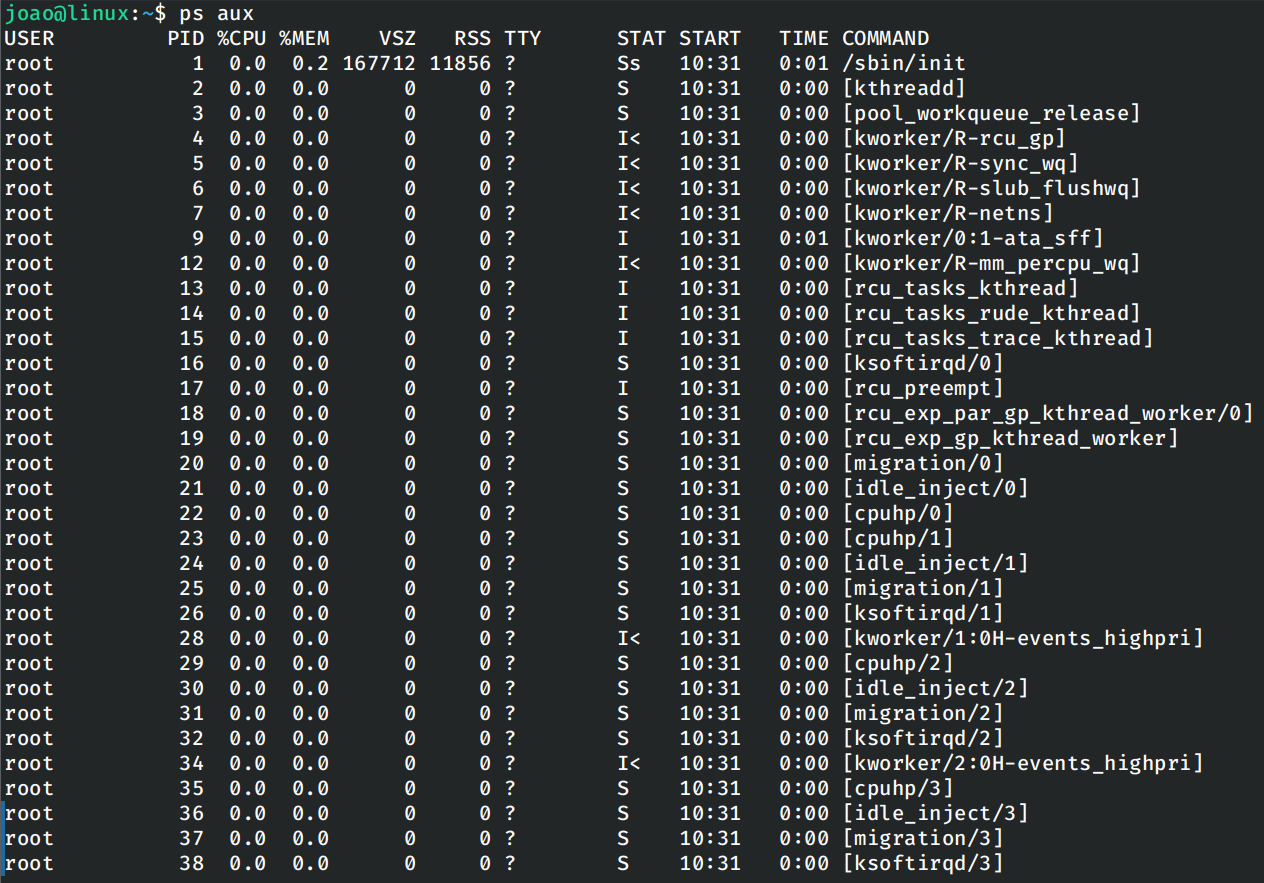
\includegraphics[scale=0.45]{figuras/ps.png}
  \caption{Saída do comando \textit{ps aux}.}
  \label{fig:ps}
\end{figure}

O comando \textit{ps aux}, apresenta as seguintes colunas~\cite{shotts2017}:

\begin{itemize}
    \item \textbf{USER:} Descreve o usuário que é dono deste processo.
    
    \item \textbf{PID:} \textit{Process ID} é o identificador númerico deste processo que está executando no sistema. Usado para o controle do processo no sistema operacional.
    \item \textbf{\%CPU:} A porcentagem de tempo em execução durante todo o tempo de vida de um processo.
    
    \item \textbf{\%MEM:} Total de memória ocupada pelo processo, expresso em porcentagem.
    
    \item \textbf{VSZ:} Quantidade total de memória virtual alocada para o processo.
    
    \item \textbf{RSS:} Quantidade de memória física que um processo está utilizando ativamente no momento, excluindo a memória que está em \textit{swap}.
    
    \item \textbf{TTY:} Terminal de controle associado a este processo. Processos que não possuem um terminal associado, como \textit{daemons}, sendo representados com o símbolo ``?'', caso contrário o nome do terminal de controle irá aparecer.
    
    \item \textbf{STAT:} Descreve o estado do processo. Alguns dos estados comumente encontrados são:
    
    \begin{itemize}
        \item \textbf{D:} \textit{Uninterruptible sleep}, o processo está esperando por uma operação de entrada/saída e não pode ser interrompido.
        \item \textbf{I:} \textit{Idle kernel thread}, o processo é uma \textit{thread} do núcleo que está ociosa, aguardando trabalho.
        \item \textbf{R:}\textit{Running} ou \textit{runnable}, o processo está em execução ou está pronto para ser executado.
        \item \textbf{S:} \textit{Interruptible sleep}, o processo está esperando por um evento para completar e pode ser interrompido por sinais.
        \item \textbf{Z:} \textit{Defunct (``zombie'')}, o processo foi terminado, mas não foi ``recolhido'' pelo seu processo pai.
    \end{itemize}
    
    \item \textbf{START:} Indica o tempo que o processo foi iniciado.
    
    \item \textbf{TIME:} Indica o tempo total de CPU que o processo consumiu desde sua inicialização.
    
    \item \textbf{COMMAND:} Exibe o nome do comando que está sendo executado pelo processo.
\end{itemize}

Os processos de usuário podem ser facilmente identificados pelo nome do usuário que os possui; a Figura~\ref{fig:user} ilustra a saída com alguns desses processos. Já os \textit{daemons}, que geralmente são iniciados com o sistema operacional, podem ser um pouco mais difíceis de identificar. No entanto, é comum que seus nomes terminem com a letra ``d'', o que pode ser observado na Figura~\ref{fig:daemon}~\cite{negus2012}.

\begin{figure}[H]
  \centering
  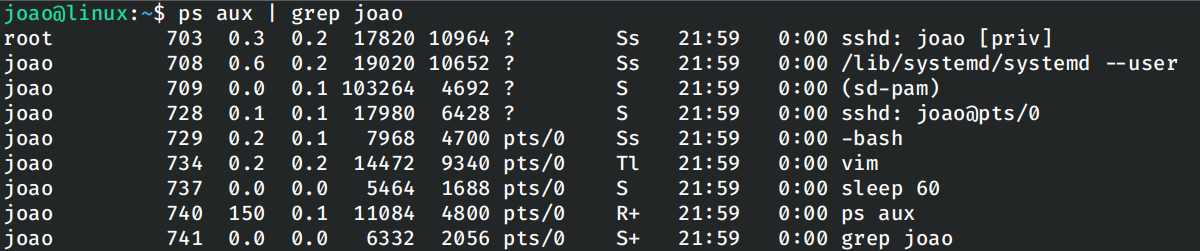
\includegraphics[scale=0.45]{figuras/user.png}
  \caption{Processo de usuário.}
  \label{fig:user}
\end{figure}

\begin{figure}[H]
  \centering
  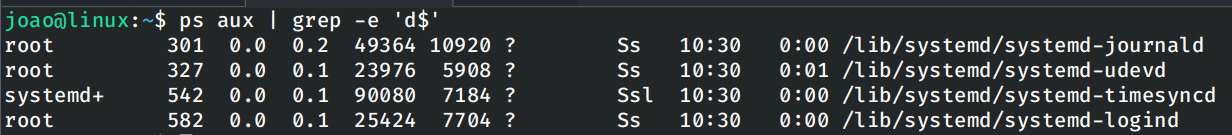
\includegraphics[scale=0.45]{figuras/daemons.png}
  \caption{Processo de sistema.}
  \label{fig:daemon}
\end{figure}

\subsection{Processos \textit{zombie}}
\label{subsec:zombie}

Um processo está no estado \textit{zombie} quando já concluiu sua execução, mas o sistema ainda não liberou os recursos que lhe foram alocados~\cite{stallings2018}. Por vezes em um processo em execução, ocorre do processo que é denominado ``pai'' criar um processo ``filho'' e esperar que este termine sua execução, usualmente com o comando \textit{wait} (em sistemas UNIX). O estado \textit{zombie} se faz necessário, pois o processo pai pode precisar da saída do processo filho para continuar sua execução. O pai só consegue acessar essa informação se o processo filho permanecer na tabela de processos do sistema operacional.

Assim, um processo em estado zumbi é equivalente a um processo que já foi concluído. Por esse motivo, ele não pode ser afetado por sinais como o \textit{SIGKILL}, que pode ser enviado a um processo por meio do comando \texttt{kill -SIGKILL pid}, onde \textit{pid} é o identificador do processo. A Figura~\ref{fig:kill} ilustra um programa que recebeu o sinal \textit{SIGKILL} e foi finalizado, enquanto a Figura~\ref{fig:zombie} mostra um processo que recebeu o mesmo sinal, mas por estar no estado \textit{zombie} continuou na tabela de processos.

\begin{figure}[H]
  \centering
  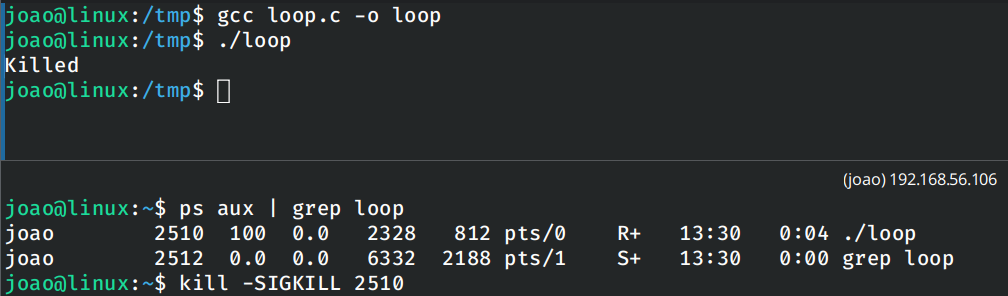
\includegraphics[scale=0.45]{figuras/kill.png}
  \caption{Comando \textit{kill} em um processo executando.}
  \label{fig:kill}
\end{figure}

\begin{figure}[H]
  \centering
  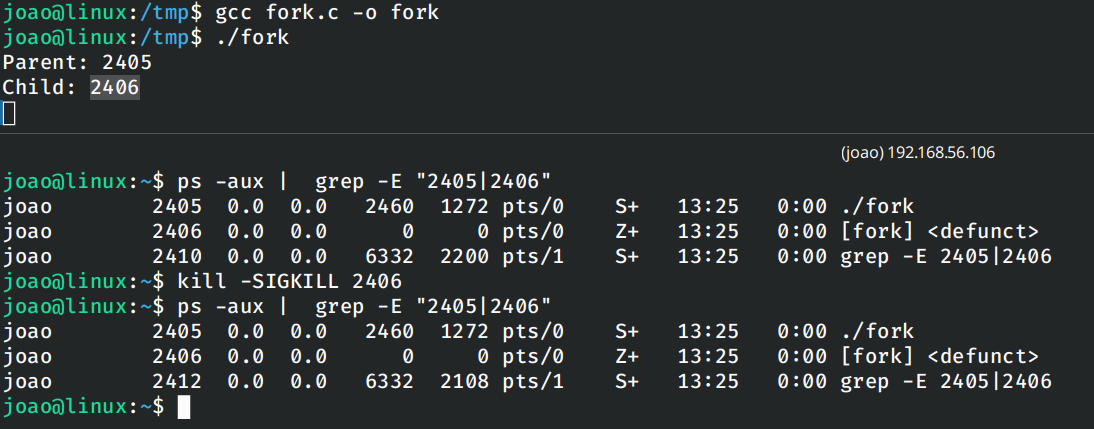
\includegraphics[scale=0.45]{figuras/zombie.png}
  \caption{Comando \textit{kill} em um processo \textit{zombie}.}
  \label{fig:zombie}
\end{figure}

\subsection{Suspendendo Processos}
\label{subsec:suspendendo}

O comando \textit{kill} pode ser utilizado para enviar sinais a processos em execução, sinais como \textit{STOP} e \textit{CONT} podem ser usados junto a este comando para suspender ou retomar a execução de um processo~\cite{guiafoca}. A Figura~\ref{fig:interrupt} mostra o código sendo executado, já a  Figura~\ref{fig:signal} mostra o uso do \textit{kill} com os sinais para suspender e retomar a execução do processo.

\begin{figure}[H]
  \centering
  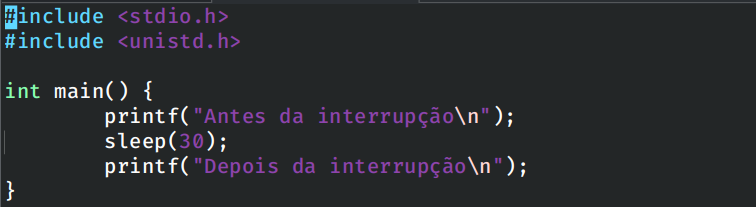
\includegraphics[scale=0.45]{figuras/interrupt.png}
  \caption{Código para demonstração da interrupção.}
  \label{fig:interrupt}
\end{figure}

\begin{figure}[H]
  \centering
  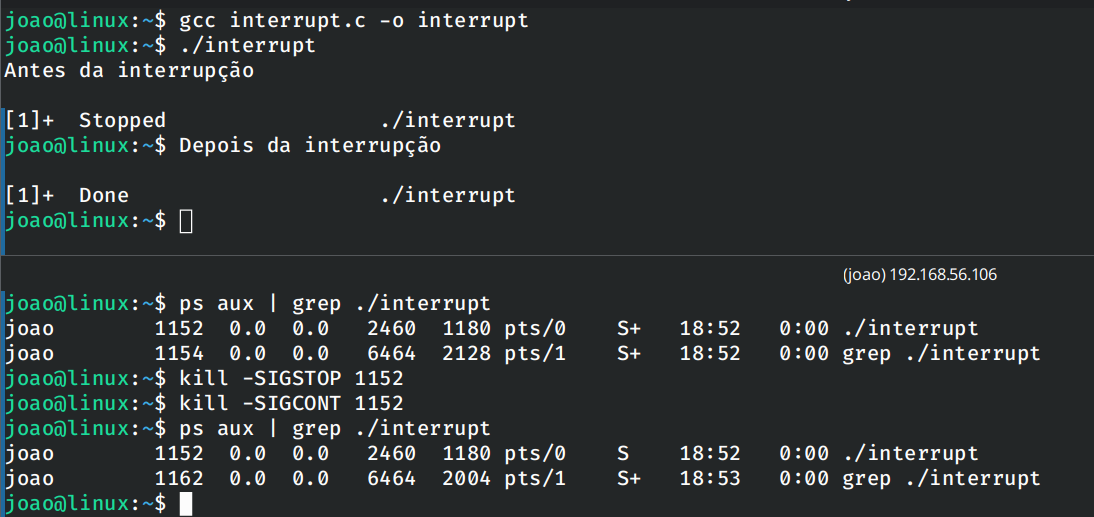
\includegraphics[scale=0.45]{figuras/signal.png}
  \caption{Comando \textit{kill} com sinais \textit{STOP} e \textit{CONT} em um processo executando.}
  \label{fig:signal}
\end{figure}

Outra forma de suspender um processo em execução é utilizando o comando \textit{Ctrl+Z}, que o coloca em segundo plano. Para listar os processos em segundo plano, podemos usar o comando \textit{jobs}. Para retomar um processo colocado em segundo plano, utilizamos o comando \textit{fg}, que traz o processo de volta ao primeiro plano. A Figura~\ref{fig:background} ilustra o uso de cada um desses comandos.

\begin{figure}[H]
  \centering
  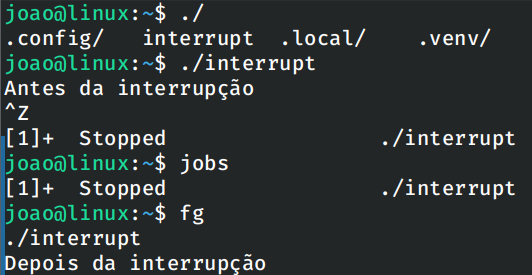
\includegraphics[scale=0.45]{figuras/background.png}
  \caption{Saída dos comandos de suspensão e retomada da execução de processos.}
  \label{fig:background}
\end{figure}

\subsection{Utilização de Recursos do Sistema}
\label{subsec:recursos}

Na máquina virtual analisada, não houve uso significativo de recursos de CPU, memória ou tempo, evidenciando um desempenho estável e eficiente do sistema. A Figura~\ref{fig:cpu}, Figura~\ref{fig:mem} e a Figura~\ref{fig:time} ilustram, respectivamente, a utilização de CPU, memória e tempo de execução do sistema.

\begin{figure}[H]
  \centering
  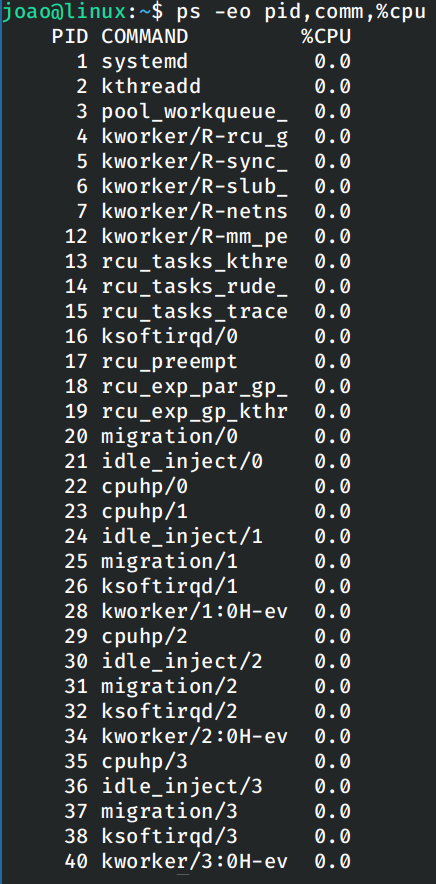
\includegraphics[scale=0.45]{figuras/cpu.png}
  \caption{Uso de CPU pelos processos do sistema.}
  \label{fig:cpu}
\end{figure}

\begin{figure}[H]
  \centering
  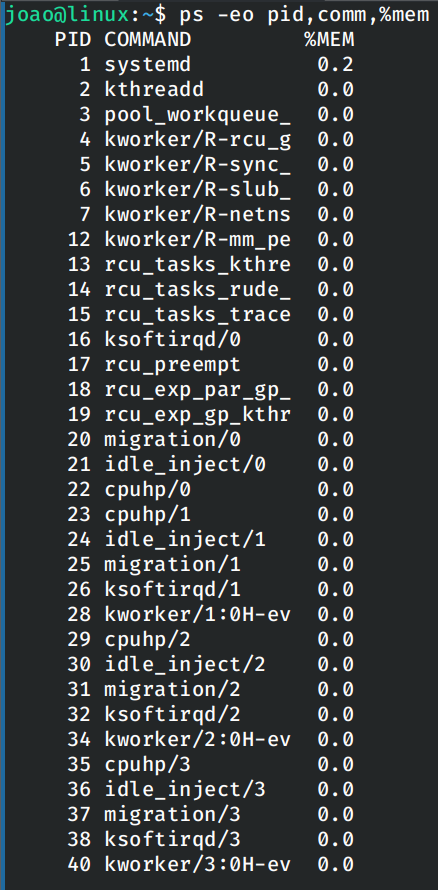
\includegraphics[scale=0.45]{figuras/mem.png}
  \caption{Uso de memória pelos processos do sistema.}
  \label{fig:mem}
\end{figure}

\begin{figure}[H]
  \centering
  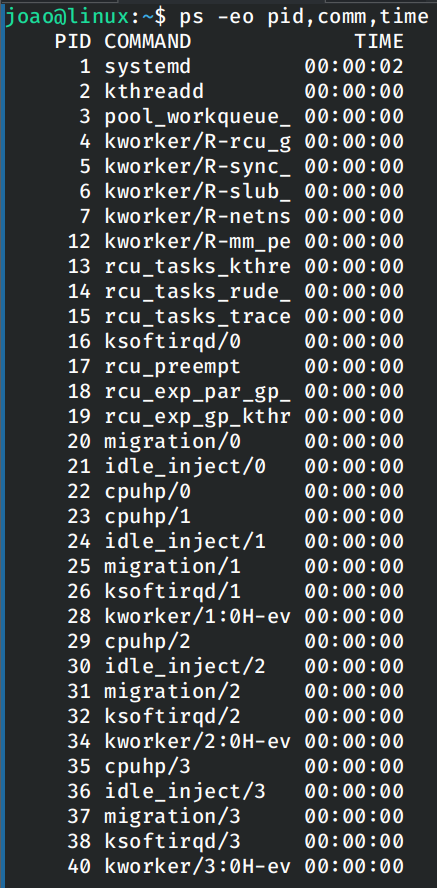
\includegraphics[scale=0.45]{figuras/time.png}
  \caption{Tempo de execução dos processos do sistema.}
  \label{fig:time}
\end{figure}

\subsection{\textit{fork} Recursivo}
\label{subsec:fork}

O código apresentado na Figura~\ref{fig:fork} foi desenvolvido para demonstrar os efeitos da criação de processos filhos de maneira recursiva e sem controle. Ao ser executado ocorre um crescimento exponencial na quantidade de processos do sistema. Essa expansão contínua consome recursos que precisam ser alocados para cada um dos processos criados, levando a um esgotamento de recursos e degradação do desempenho do sistema, em certo momento durante a prática o sistema precisou ser desligado, pois o mesmo já não estava mais respondendo.

\begin{figure}[H]
  \centering
  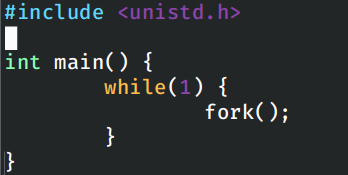
\includegraphics[scale=0.5]{figuras/fork.png}
  \caption{Código de criação recursiva de processos.}
  \label{fig:fork}
\end{figure}

A Figura~\ref{fig:ulimit} exibe a saída do comando \texttt{ulimit -a}, que detalha os limites de uso dos recursos do sistema. Nela, podemos observar que o sistema tem um limite máximo de 15.587 processos. 

\begin{figure}[H]
  \centering
  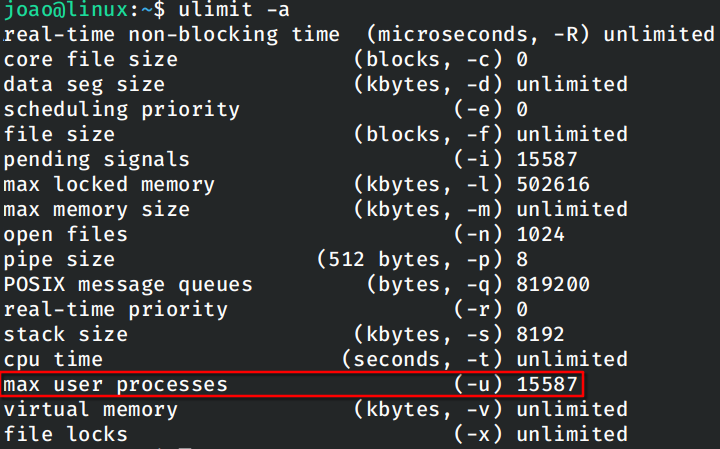
\includegraphics[scale=0.5]{figuras/ulimit.png}
  \caption{Verificação de limites de recursos do sistema.}
  \label{fig:ulimit}
\end{figure}

A Figura~\ref{fig:bomb} demonstra os efeitos dessa criação desenfreada de processos no sistema. Após a execução do programa que cria processos filhos de maneira recursiva, o sistema chegou no seu limite máximo de processos e não foi mais possível executar nenhum outro tipo de comando, impedindo até mesmo a utilização do comando \textit{ps} para visualização dos processos no sistema. O que evidencia o como este tipo de programa afeta negativamente o sistema operacional.

\begin{figure}[H]
  \centering
  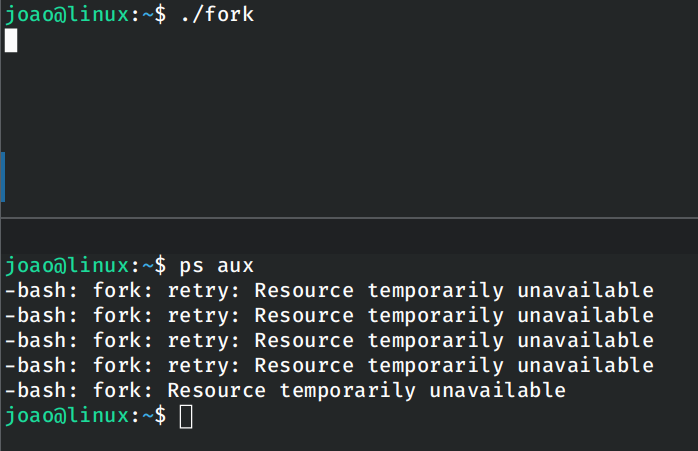
\includegraphics[scale=0.5]{figuras/bomb.png}
  \caption{Execução do programa que cria processos recursivamente.}
  \label{fig:bomb}
\end{figure}

\section{Discussão dos Resultados}
\label{sec:discussao}

FAZER

\section{Conclusões}
\label{sec:conclusoes}

FAZER

% ----------------------------------------------------------
% ELEMENTOS PÓS-TEXTUAIS
% ----------------------------------------------------------
\postextual
% ----------------------------------------------------------
% Referências bibliográficas
% ----------------------------------------------------------
\renewcommand{\bibsection}{%
\section{\bibname}
\bibmark
%\ifnobibintoc\else
%\phantomsection
%\addcontentsline{toc}{section}{\bibname}
%\fi
\prebibhook}

\bibliography{abntex2-modelo-references}

\end{document}
